\section{Provas dos teoremas}
 
%%%%%%%%%%%%%%%%%%%%%%%%%%%%%%%%%%%%%%%%%%%%%%%%%%%%%%%%%%%%%%%%%%%%%%%%%%%%%%%%%%%%%%%
%%%%%%%%%%%%%%%%%%%%%%%%%%%%%%%%%%%%%%%%%%%%%%%%%%%%%%%%%%%%%%%%%%%%%%%%%%%%%%%%%%%%%%%
\begin{myproofT}[Prova do Teorema \ref{theo:minhxhx}]\label{proof:theo:minhxhx}
Dados,
um escalar $x \in \mathbb{R}$, 
um escalar $a \in \mathbb{R}$,  
uma função $h:\mathbb{R} \rightarrow \mathbb{R}$, e 
definida a Eq. (\ref{eq:proof:minhxhx0}),
\begin{equation}\label{eq:proof:minhxhx0}
e(x)=||h(x)-a||^2.
\end{equation}
Para achar o valor  $\hat{x}$ que gere o menor valor de $e(x)$, é aplicado
o critério que um ponto de inflexão $x^+$ (máximo, mínimo ou ponto de sela) de $e(x)$ 
pode ser achado quando 
$\left. \frac{d e(x)}{d x }\right|_{x=x^+} \equiv e'(x^+) =0$.
Assim, 
usando o Teorema \ref{theo:derfxbCfxb0} podemos 
rescrever esta igualdade como a Eq. (\ref{eq:proof:minhxhxe}),
\begin{equation}\label{eq:proof:minhxhxe}
2  h'(x) \left[h(x) -a\right] = e'(x)=0,
\end{equation}
Da Eq. (\ref{eq:proof:minhxhxe}), observamos 
que existem duas formas de achar um ponto de inflexão $x^+$,
\begin{itemize}
 \item a primeira forma a achamos se temos um valor $x^+$ tal que $h'(x^+)=0$, 
que representa um ponto de inflexão simultâneo em $e(x)$ e $h(x)$, e
 \item a segunda forma é achando um valor $x^+$ tal que $h(x^+)=a$;
que representa um ponto de inflexão de $e(x)$, mas não
necessariamente de $h(x)$; 
sendo este ponto $x^+=\hat{x}$ também um mínimo absoluto, pois provocam $e(\hat{x})=0$.
\end{itemize}




Por outro lado, podemos realizar uma aproximação linear de $h(x)$ em $e(x)$
ao redor do ponto $p$, usando a \hyperref[def:taylor]{\textbf{serie de Taylor}},
de modo que a Eq. (\ref{eq:proof:minhxhx0}) pode ficar expressada como
\begin{equation}\label{eq:proof:minhxhxe:approx0}
e(x) \approx  e_p(x) = ||h'(p)\{x-p\}-\{a-h(p)\}||^2.
\end{equation}
Assim, da Eq. (\ref{eq:proof:minhxhxe:approx0})
podemos concluir que um ponto $x^*$ que é 
um mínimo da aproximação linear $e_p(x)$ feita em $e(x)$ ao redor do ponto $p$,
pode ser achado como
\begin{equation}\label{eq:proof:minhxhx2}
 h'(p)\{x^*-p\} = \{a-h(p)\} \qquad \leftrightarrow \qquad x^* = p - \frac{h(p)-a}{ h'(p)}.
\end{equation} 

Desta equação podemos tirar a seguintes conclusões:
\begin{itemize}

\item Observamos que a posição $p$ é corregida para ficar próximo à posição $x^*$, 
que é um mínimo absoluto de $e_p(x)$ na direção de um mínimo (qualquer) de $e(x)$;
pelo que se deduz que a Eq. (\ref{eq:proof:minhxhx2})
pode ser usada para procurar aproximações $x^*$ de pontos mínimos $\hat{x}$ em $e(x)$ desde a posição $p$;
ou pelo menos aproximações de novas posições em caminhos numa direção descendente de $e(x)$.

\item A Eq. (\ref{eq:proof:minhxhx2}) é satisfeita 
com $x^* \approx p$ se acharmos um  
ponto $p$ onde  $a \approx h(p)$; 
é dizer um mínimo global de $e(x)$ em $p$.%, como pode ser visto na Figura \ref{fig:ex0a}. 

\item Dado que a Eq. (\ref{eq:proof:minhxhx2}) tem um termo $h'(p)$ no denominador,
valores $p$ que cumpram $h'(p)\approx 0$ provocam uma correção distante (divergência) da posição $p$,
nos casos onde $p$ se aproxime a máximos e pontos de sela,
ou mínimos locais. 
Mas sim se trata de um mínimo global com $h(p)\approx a$, 
o comportamento será inesperado e dependerá se é finito ou não, o
\begin{equation}
lim_{x\rightarrow p } \frac{h(p)-a}{h'(p)}.
\end{equation}

\item Se modificamos a Eq. (\ref{eq:proof:minhxhx2}), e escolhemos um ponto  
$p_0$ que consideremos próximo ao ponto $\hat{x}$ que minimiza $e(\hat{x})$,
podemos achar iterativamente aproximações lineares $x^*$ cada vez mais próximos a  $\hat{x}$,
se usamos a seguinte equação iterativa,
\begin{equation}\label{eq:proof:minhxhx3}
p_{k} \leftarrow p_{k-1} - \frac{ h(p_{k-1})-a}{h'(p_{k-1})},
\end{equation}
iniciando desde um $p_{0}$ 
ate que exista uma tendencia prolongada onde se observe que $p_{k}$ é muito próximo a $p_{k-1}$,
momento no qual declaramos que $\hat{x} \approx p_{k}$.
\item Pode existir um mínimo global $\hat{x}$ de $e(\hat{x})>0$.
Isto nos restringe a que no uso da Eq. (\ref{eq:proof:minhxhx3}),
nosso critério principal para estabelecer o final do cáculo iterativo,
deve ser a tendencia na  proximidade entre $p_{k}$ e $p_{k-1}$ 
e não o valor de $e(x_k)$.
\end{itemize}

Um diagrama completo resumindo todas estas conclusões pode ser visto na Figura \ref{fig:fluxohx1}.
\end{myproofT}



\begin{figure}[!h]
     \centering
         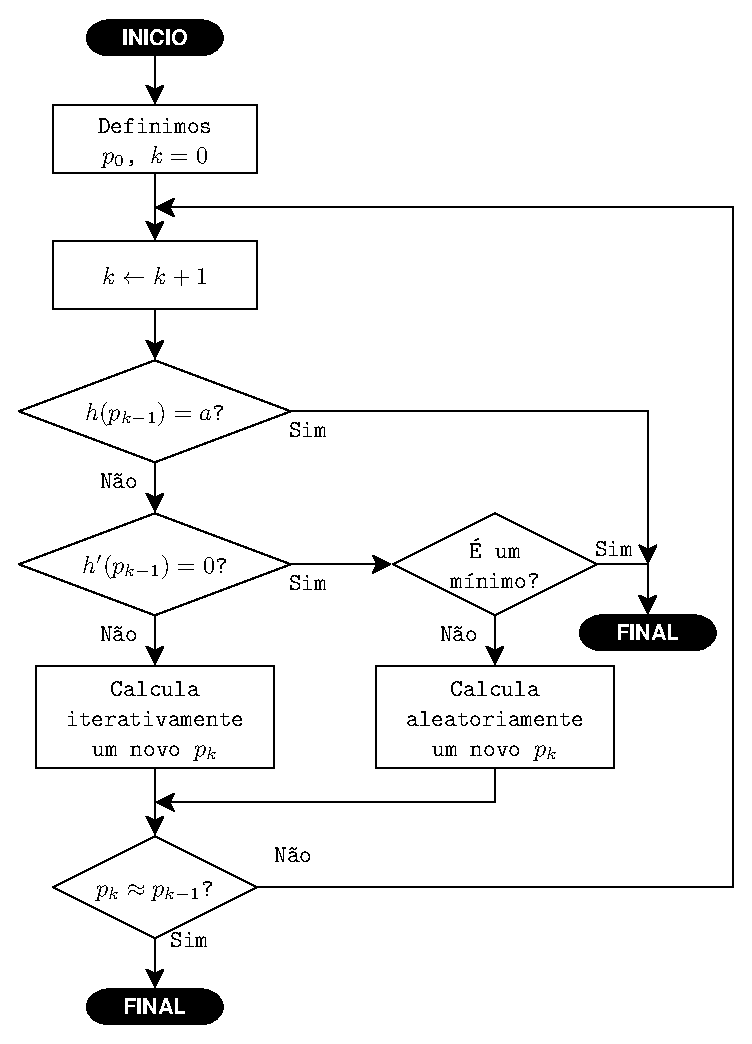
\includegraphics[width=0.75\textwidth]{chapters/minimization-hx/fluxo1.eps}
        \caption{Diagrama de fluxo da solução iterativa para achar um mínimo, seguindo a Prova \ref{proof:theo:minhxhx}.}
        \label{fig:fluxohx1}
\end{figure}


%%%%%%%%%%%%%%%%%%%%%%%%%%%%%%%%%%%%%%%%%%%%%%%%%%%%%%%%%%%%%%%%%%%%%%%%%%%%%%%%%%%%%%%
%%%%%%%%%%%%%%%%%%%%%%%%%%%%%%%%%%%%%%%%%%%%%%%%%%%%%%%%%%%%%%%%%%%%%%%%%%%%%%%%%%%%%%%
\begin{myproofT}[Prova do Teorema \ref{theo:minhxhxxbxb}]\label{proof:theo:minhxhxxbxb}

Dados,
um escalar $x \in \mathbb{R}$, 
um escalar $a \in \mathbb{R}$,
um escalar $\alpha \in \mathbb{R}^{+}$,
um escalar $b \in \mathbb{R}$,
uma função $h:\mathbb{R} \rightarrow \mathbb{R}$, e 
definida a Eq. (\ref{eq:proof:minhxhxxbxb0}),
\begin{equation}\label{eq:proof:minhxhxxbxb0}
e(x)=||h(x)-a||^2+\alpha ||x-b||^2.
\end{equation}

Para achar o valor  $\hat{x}$ que gere o menor valor de $e(x)$, é aplicado
o critério que um ponto de inflexão $x^+$ (máximo, mínimo ou ponto de sela) de $e(x)$ 
pode ser achado quando 
$\left. \frac{d e(x)}{d x }\right|_{x=x^+} \equiv e'(x^+) =0$.
Assim, 
usando o Teorema \ref{theo:derfxbCfxb0} e \ref{theo:derAxbAxb}  podemos 
rescrever esta igualdade como a Eq. (\ref{eq:proof:minhxhxxbxbe}),
\begin{equation}\label{eq:proof:minhxhxxbxbe}
2  h'(x) \left[h(x) -a\right]+2\alpha (x-b)= e'(x)=0,
\end{equation}
Da Eq. (\ref{eq:proof:minhxhxxbxbe}), observamos 
que existem duas formas de achar um ponto de inflexão $x^+$,
\begin{itemize}
 \item a primeira forma a achamos se temos um valor $x^+=b$ tal que $h'(b)=0$, 
que representa um ponto de inflexão simultâneo em $e(x)$ e $h(x)$, e
 \item a segunda forma é achando um valor $x^+=b$ tal que $h(b)=a$;
que representa um ponto de inflexão de $e(x)$, mas não
necessariamente de $h(x)$; 
sendo este ponto $x^+=\hat{x}=b$ também um mínimo absoluto, pois provocam $e(\hat{x})=0$.
\end{itemize}

Por outro lado, podemos realizar uma aproximação linear de $h(x)$ em $e(x)$
ao redor do ponto $p$, usando a \hyperref[def:taylor]{\textbf{serie de Taylor}},
de modo que a Eq. (\ref{eq:proof:minhxhxxbxb0}) pode ficar expressada como
\begin{equation}\label{eq:proof:minhxhxxbxbe:approx0}
e(x) \approx  e_p(x) = ||h'(p)\{x-p\}-\{a-h(p)\}||^2+\alpha ||x-b||^2.
\end{equation}
Assim, da Eq. (\ref{eq:proof:minhxhxxbxbe:approx0})
podemos concluir que um ponto $x^*$ que é 
o mínimo da aproximação linear $e_p(x)$ feita em $e(x)$ ao redor do ponto $p$,
pode ser achado aplicando $\left. \frac{d e_p(x)}{d x }\right|_{x=x^*} \equiv e_{p}'(x^*) =0$,
de modo que obtemos
\begin{equation}\label{eq:proof:minhxhxaxb2a}
 2 h'(p)[h'(p)\{x^*-p\} -\{a-h(p)\}] + \alpha [x^*-b] = 0,
\end{equation} 
\begin{equation}\label{eq:proof:minhxhxaxb2}
x^* = p - \frac{h'(p)\{h(p)-a\}+\alpha\{p-b\}}{ h'(p)^2+\alpha}.
\end{equation} 

Desta equação podemos tirar a seguintes conclusões:


\begin{itemize}

\item Observamos que a posição $p$ é corregida para ficar próximo à posição $x^*$, 
que é um mínimo absoluto de $e_p(x)$ na direção de um mínimo (qualquer) de $e(x)$;
pelo que se deduz que a Eq. (\ref{eq:proof:minhxhxaxb2})
pode ser usada para procurar aproximações $x^*$ de pontos mínimos $\hat{x}$ em $e(x)$ desde a posição $p$;
ou pelo menos aproximações de novas posições em caminhos numa direção descendente de $e(x)$.

\begin{comment}
\item A Eq. (\ref{eq:proof:minhxhxaxb2}) é satisfeita 
com $x^* \approx p$ se acharmos um  
ponto $p=b$ onde  $a \approx h(b)$; 
é dizer um mínimo global de $e(x)$ em $b$.%, como pode ser visto na Figura \ref{fig:ex0a}. 
\item A Eq. (\ref{eq:proof:minhxhxaxb2}) é satisfeita 
com $x^* \approx p$ se acharmos um  
ponto $p=b$ onde  $0 \approx h'(b)$; 
é dizer um ponto de inflexão de $e(x)$ em $b$.
\end{comment}

\item Se reescrevemos a Eq. (\ref{eq:proof:minhxhxaxb2}) usando o Teorema \ref{theo:derfxbCfxb0}
e o Corolário \ref{coro:derAxbAxb2},
obtemos
\begin{equation}\label{eq:proof:minhxhxaxbea1}
x^* \approx p -
\frac{ e'(p)}{2 \{h'(p)^2+\alpha\} },
\end{equation}
onde a Eq. (\ref{eq:proof:minhxhxaxbea1}) é satisfeita 
com $x^* \approx p$
se acharmos um  ponto $p$ onde  
$e'(p)\approx 0$; 
é dizer $p$ é um ponto de inflexão de $e(x)$, como já foi analisado na Eq. (\ref{eq:proof:minhxhxxbxbe}).
%como pode ser visto na Figura \ref{fig:ex0b}.
Porém, dado que a Eq. (\ref{eq:proof:minhxhxaxbea1}) avança desde $p$ na direção de um mínimo $x^*$, 
mesmo que nos pontos de inflexão correspondentes a máximos ou pontos de sela,
encontremos valores de $p$ próximos a $x^*$,
 estes casos serão pouco estáveis pois
a correção da posição $p$ será na direção de um mínimo e não do máximo.

\item Se modificamos a Eq. (\ref{eq:proof:minhxhxaxb2}), e escolhemos um ponto  
$p_0$ que consideremos próximo ao ponto $\hat{x}$ que minimiza $e(\hat{x})$,
podemos achar iterativamente aproximações lineares $x^*$ cada vez mais próximos a  $\hat{x}$,
se usamos a seguinte equação iterativa,
\begin{equation}\label{eq:proof:minhxhxaxb3}
p_{k} \leftarrow p_{k-1} - \frac{ h'(p_{k-1})\{h(p_{k-1})-a\}+\alpha\{p-b\}}{h'(p_{k-1})^2+\alpha},
\end{equation}
iniciando desde um $p_{0}$ 
ate que exista uma tendencia prolongada onde se observe que $p_{k}$ é muito próximo a $p_{k-1}$,
momento no qual declaramos que $\hat{x} \approx p_{k}$.
\item Pode existir um mínimo global $\hat{x}$ de $e(\hat{x})>0$.
Isto nos restringe a que no uso da Eq. (\ref{eq:proof:minhxhxaxb3}),
nosso critério principal para estabelecer o final do cáculo iterativo,
deve ser a tendencia na  proximidade entre $p_{k}$ e $p_{k-1}$ 
e não o valor de $e(x_k)$.
\end{itemize}

Um diagrama completo resumindo todas estas conclusões pode ser visto na Figura \ref{fig:fluxohx2}.
\end{myproofT}



\begin{figure}[!h]
     \centering
         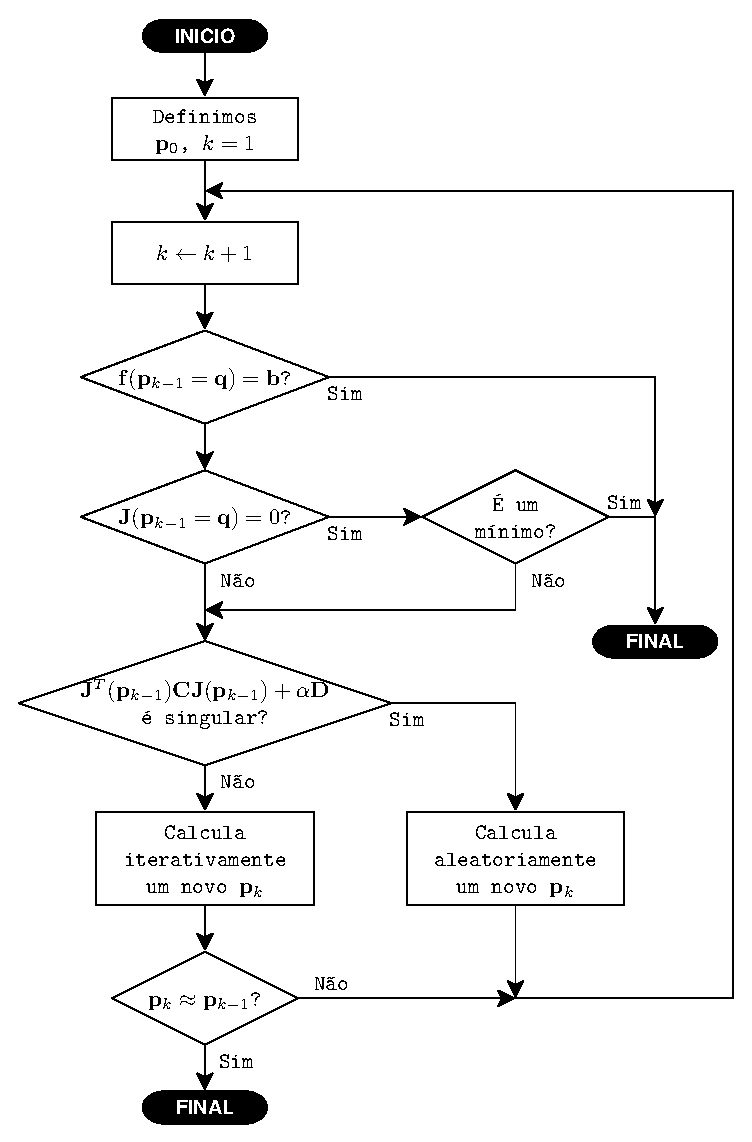
\includegraphics[width=0.75\textwidth]{chapters/minimization-hx/fluxo2.eps}
        \caption{Diagrama de fluxo da solução iterativa para achar um mínimo, seguindo a Prova \ref{proof:theo:minhxhxxbxb}.}
        \label{fig:fluxohx2}
\end{figure}


%%%%%%%%%%%%%%%%%%%%%%%%%%%%%%%%%%%%%%%%%%%%%%%%%%%%%%%%%%%%%%%%%%%%%%%%%%%%%%%%%%%%%%%
%%%%%%%%%%%%%%%%%%%%%%%%%%%%%%%%%%%%%%%%%%%%%%%%%%%%%%%%%%%%%%%%%%%%%%%%%%%%%%%%%%%%%%%
\begin{myproofT}[Prova do Teorema \ref{theo:minhxhxxoxo}]\label{proof:theo:minhxhxaxoxo}

Dados,
um escalar $x \in \mathbb{R}$, 
um escalar $a \in \mathbb{R}$,
um escalar $\alpha \in \mathbb{R}^{+}$,
um escalar $x_{last} \in \mathbb{R}$,
uma função $h:\mathbb{R} \rightarrow \mathbb{R}$, e 
definida a Eq. (\ref{eq:proof:minhxhxxoxo0}),
\begin{equation}\label{eq:proof:minhxhxxoxo0}
e(x)=||h(x)-a||^2+\alpha ||x-x_{last}||^2.
\end{equation}
tendo em consideração que $x_{last}$ é uma constante equivalente a $x_{k-1}$
numa busca iterativa ou equivalente a $p$, 
se decidimos usar uma aproximação linear ao redor de $p$ em $h(x)$; 
é dizer, o segundo somando na Eq. (\ref{eq:proof:minhxhxxoxo0}) 
procura minimizar $||x_{k}-x_{k-1}||^2$.


Para achar o valor  $\hat{x}$ que gere o menor valor de $e(x)$, é aplicado
o critério que um ponto de inflexão $x^+$ (máximo, mínimo ou ponto de sela) de $e(x)$ 
pode ser achado quando 
$\left. \frac{d e(x)}{d x }\right|_{x=x^+} \equiv e'(x^+) =0$.
Assim, 
usando o Teorema \ref{theo:derfxbCfxb0} e \ref{theo:derAxbAxb}  podemos 
rescrever esta igualdade como a Eq. (\ref{eq:proof:minhxhxxoxoe}),
\begin{equation}\label{eq:proof:minhxhxxoxoe}
2  h'(x) \left[h(x) -a\right]+2\alpha (x-x_{last})= e'(x)=0,
\end{equation}
Da Eq. (\ref{eq:proof:minhxhxxoxoe}), observamos 
que existem duas formas de achar um ponto de inflexão $x^+$,
\begin{itemize}
 \item a primeira forma a achamos se temos um valor $x^+=x_{last}$ tal que $h'(x_{last})=0$, 
que representa um ponto de inflexão simultâneo em $e(x)$ e $h(x)$, e
 \item a segunda forma é achando um valor $x^+=x_{last}$ tal que $h(x_{last})=a$;
que representa um ponto de inflexão de $e(x)$, mas não
necessariamente de $h(x)$; 
sendo este ponto $x^+=\hat{x}=x_{last}$ também um mínimo absoluto, pois provocam $e(\hat{x})=0$.
\end{itemize}

Por outro lado, procurando outros critérios para achar os pontos de inflexão,
podemos igualar $x_{last}\equiv p$ e 
realizar uma aproximação linear de $h(x)$ em $e(x)$
ao redor do ponto $p$ usando a \hyperref[def:taylor]{\textbf{serie de Taylor}},
de modo que a Eq. (\ref{eq:proof:minhxhxxoxo0}) pode ficar expressada como
\begin{equation}\label{eq:proof:minhxhxxoxo0approx}
e(x) \approx e_{p}(x)  \equiv ||h'(p)[x-p]-[a-h(p)]||^2+\alpha||x-p||^2,
\end{equation}


%%%%%%%
Assim, usando o resultado da Prova \ref{proof:theo:minAxbCAxbalphaxqD} na Eq. (\ref{eq:proof:minhxhxxoxo0approx}), 
podemos concluir que um ponto $x^*$ que é 
o mínimo da aproximação linear $e_p(x)$ feita em $e(x)$ ao redor do ponto $p$,
pode ser achado aplicando $\left. \frac{d e_p(x)}{d x }\right|_{x=x^*} \equiv e_{p}'(x^*) =0$,
de modo que obtemos
\begin{equation}\label{eq:proof:minhxhxaxo2a}
 2 h'(p)[h'(p)\{x^*-p\} -\{a-h(p)\}] + \alpha [x^*-p] = 0,
\end{equation} 
\begin{equation}\label{eq:proof:minhxhxaxo2}
x^* = p - \frac{h'(p)\{h(p)-a\}}{ h'(p)^2+\alpha}.
\end{equation} 








Desta equação podemos tirar a seguintes conclusões:
\begin{itemize}

\item Observamos que a posição $p$ é corregida para ficar próximo à posição $x^*$, 
que é o valor mínimo na aproximação linear ao redor de $p$;
pelo que se deduz que a Eq. (\ref{eq:proof:minhxhxaxo2})
pode ser usada para procurar aproximações de pontos mínimos $\hat{x}$ em $e(x)$ desde a posição $p$,
ou pelo menos aproximações de novas posições em caminhos numa direção descendente de $e(x)$.

\begin{comment}
\item A Eq. (\ref{eq:proof:minhxhxaxo2}) é satisfeita 
com $x^* \approx p$ se acharmos um  
ponto $p$ onde  $a \approx h(p\approx x_{last})$; 
é dizer um mínimo global de $e(x)$ em $p$. 
\end{comment}

\item Se reescrevemos a Eq. (\ref{eq:proof:minhxhxaxo2}) usando o Teorema \ref{theo:derfxbCfxb0}
e o Corolário \ref{coro:derAxbAxb2},
obtemos
\begin{equation}\label{eq:proof:minhxhxaxoxo2ea1}
x^* \approx p - \frac{ e'(p)}{2(h'(p)^2+\alpha)},
\end{equation}
onde a Eq. (\ref{eq:proof:minhxhxaxoxo2ea1}) é satisfeita 
com $x^* \approx p$
se acharmos um  ponto $p$ onde  
$e'(p)\approx 0$; 
é dizer $p$ é um ponto de inflexão de $e(x)$, como pode ser visto na Eq. (\ref{eq:proof:minhxhxxoxoe}).
Porém, dado que a Eq. (\ref{eq:proof:minhxhxaxoxo2ea1}) avança desde $p$ na direção de um mínimo $x^*$, 
mesmo que nos pontos de inflexão correspondentes a máximos ou pontos de sela,
encontremos valores de $p$ próximos a $x^*$,
 estes casos serão pouco estáveis pois
a correção da posição $p$ será na direção de um mínimo e não do máximo.

\item Se modificamos a Eq. (\ref{eq:proof:minhxhxaxo2}), e escolhemos um ponto  
$p_0$ que consideremos próximo ao ponto $\hat{x}$ que minimiza $e(\hat{x})$,
podemos achar iterativamente aproximações lineares $x^*$ cada vez mais próximos a  $\hat{x}$,
se usamos a seguinte equação iterativa,
\begin{equation}\label{eq:proof:minhxhxaxoxo3b}
p_{k} \leftarrow p_{k-1} - \frac{h'(p_{k-1})\{h(p_{k-1})-a\}}{h'(p_{k-1})^2 +\alpha},
\end{equation}
onde se inicia desde um $p_{0}$ 
ate que exista uma tendencia prolongada onde se observe que $p_{k}$ é muito próximo a $p_{k-1}$,
momento no qual declaramos que $\hat{x} \approx p_{k}$.
Disto também se deduz que o erro a minimizar em cada iteração será diferente e influenciado pelo valor do ponto $p_{k-1}$,
\begin{equation}
e_{k-1}(x)  \equiv ||h(x)-a||^2+\alpha||x-p_{k-1}||^2
\end{equation}
\item Pode existir um mínimo global $\hat{x}$ de $e(\hat{x}) > 0$.
Isto nos restringe a que no uso da Eq. (\ref{eq:proof:minhxhxaxoxo3b}),
nosso critério principal para estabelecer o final do cáculo iterativo,
deve ser a tendencia na  proximidade entre $p_{k}$ e $p_{k-1}$ 
e não o valor de $e(x_k)$.
\end{itemize}~

Um diagrama completo resumindo todas estas conclusões pode ser visto na Figura \ref{fig:fluxohx3}.
\end{myproofT}
\begin{figure}[!h]
     \centering
         \includegraphics[width=0.75\textwidth]{chapters/minimization-hx/fluxo3.eps}
        \caption{Diagrama de fluxo da solução iterativa para achar um mínimo, seguindo a Prova \ref{proof:theo:minhxhxaxoxo}.}
        \label{fig:fluxohx3}
\end{figure}
